\documentclass[CJK,xcolor=pdftex,dvipsnames,table]{beamer} %\documentclass[noindent,sans,dvips]{beamer}% voss 2005-07-02
\mode<presentation>{
\usetheme{Madrid}
\usefonttheme{default}%����ģ��
%\usecolortheme{beaver}
%\usecolortheme{albatross}
%\usecolortheme{dolphin}
}
%\setlength{\parindent}{2em}
\setlength{\parindent}{0.1cm}

%\linespread{1.2}
% ������acrobat�򿪾ͻ�ȫ����ʾ
\hypersetup{pdfpagemode=FullScreen}
%\usepackage{pgf,pgfrcs,pgfarrows,pgfnodes,pgfautomata,pgfheaps,pgfshade}
\usepackage{xcolor}
%\usepackage{color}
\usepackage{colortbl}
\usepackage[english]{babel}
\usepackage{graphicx}
\usepackage{hyperref}
\hypersetup{
CJKbookmarks=true,
bookmarksnumbered=true,
bookmarksopen=true,
bookmarksopenlevel=1,
breaklinks=true,
colorlinks=true,
plainpages=false,
linkcolor=gray, %[rgb]{0.50,0.50,1.00},
pdfpagelabels,
pdfborder=0 0 0}
\urlstyle{same}
\usepackage{hypernat}

\usepackage{textcomp} %ŷԪ�ȷ���,���϶��õ�\textcelsius~%�������ڹ�ʽ����
\usepackage{amsmath,amssymb}
\usepackage{mathbbold, mathrsfs}
\usepackage[latin1]{inputenc}
\usepackage{multirow}
\usepackage{amsfonts}
\usepackage{latexsym}
\usepackage{amssymb}

%\usepackage{indentfirst}
%\usepackage{noindent}
\usepackage{mathrsfs}
\usepackage{amsmath}
\usepackage{graphicx}
\usepackage{flafter}
\usepackage{float}
%\usepackage{multimedia}
\usepackage{movie15}
%\usepackage{listings}
%\usepackage[absolute,overlay]{textpos}
\usepackage{listings}
\usepackage[timeinterval=5]{tdclock}
\usepackage{epstopdf}

%\lstloadlanguages{C}
\renewcommand{\lstlistingname}{Code}
\lstloadlanguages{C,C++,matlab,mathematica}
\lstset{language=C,tabsize=4, keepspaces=true,
    xleftmargin=2em,xrightmargin=2em, aboveskip=1em,
    %backgroundcolor=\color{lightgray},
    frame=b, %shadowbox, %none,
    keywordstyle=\color{blue}\bfseries,
    breakindent=22pt,
    numbers=left,stepnumber=1,numberstyle=\tiny,
    basicstyle=\footnotesize,
    showspaces=false,
    flexiblecolumns=true,
    breaklines=true, breakautoindent=true,breakindent=4em,
    escapeinside=``
}
\usepackage{caption}
\DeclareCaptionFont{white}{\color{white}}
\DeclareCaptionFormat{listing}{\colorbox[cmyk]{0.43, 0.35, 0.35,0.01}{\parbox{\textwidth}{#1#2#3}}}
\captionsetup[lstlisting]{format=listing,justification=raggedright,labelfont=white,textfont=white, singlelinecheck=false, margin=0pt, font={sf,bf,scriptsize}} %footnotesize
%\lstset{language=C,numbers=left,
%numberstyle= \tiny,
%keywordstyle= \color{ blue!70},commentstyle=\color{red!50!green!50!blue!50},
%frame=shadowbox,
%rulesepcolor= \color{ red!20!green!20!blue!20},escapeinside=[]
%}

%\usepackage[usenames,dvipsnames]{pstricks}
%\usepackage{pst-plot}
%\usepackage{pst-node}
%\usepackage{pst-math}

%\usepackage{bmptojpg}
%\usepackage{pstricks-add,geometry}  %confilct with algorithm2e
%\defineTColor{TRed}{red}
%\defineTColor{TGreen}{green}
%\defineTColor{TBlue}{blue}

%\usepackage{geometry}
\usepackage{CJK}

\usepackage[algo2e,ruled,linesnumbered,vlined]{algorithm2e} %conflict with pstricks-add
\newcommand{\be}{\boldsymbol{E}}
\newcommand{\beh}{\boldsymbol{E}_h}
\newcommand{\beH}{\boldsymbol{E}_H}
\newcommand{\behh}{\boldsymbol{e}_h}
\newcommand{\beI}{\boldsymbol{e}_I}
\newcommand{\tbe}{\tilde{\boldsymbol{E}}}
\newcommand{\berh}{\boldsymbol{E}_{1h}}
\newcommand{\beih}{\boldsymbol{E}_{2h}}
\newcommand{\berH}{\boldsymbol{E}_{1H}}
\newcommand{\beiH}{\boldsymbol{E}_{2H}}
\newcommand{\bh}{\boldsymbol{H}}
\newcommand{\bff}{\boldsymbol{F}}
\newcommand{\bpsi}{\boldsymbol{\psi}}
\newcommand{\bpsih}{\boldsymbol{\psi}_h}
\newcommand{\bu}{\boldsymbol{u}}
\newcommand{\buh}{\boldsymbol{u}_h}
\newcommand{\buH}{\boldsymbol{u}_H}
\newcommand{\bv}{\boldsymbol{v}}
\newcommand{\bV}{\boldsymbol{V}}
\newcommand{\bvh}{\boldsymbol{v}_h}
\newcommand{\bvH}{\boldsymbol{v}_H}
\newcommand{\bw}{\boldsymbol{w}}
\newcommand{\bW}{\boldsymbol{W}}
\newcommand{\bx}{\boldsymbol{x}}
\newcommand{\bnu}{\boldsymbol{\nu}}
\newcommand{\tu}{\tilde{\boldsymbol{u}}}
\newcommand{\tv}{\tilde{\boldsymbol{v}}}
\newcommand{\Vh}{\boldsymbol{V}_h}
\newcommand{\pih}{\boldsymbol{\Pi}_h}
\newcommand{\bwI}{\boldsymbol{w}_I}
\newcommand{\bn}{\boldsymbol{n}}
\newcommand{\bH}{\boldsymbol{H}}
\newcommand{\V}{\mathbb{V}}

\newcommand{\dx}{\mathrm{d}\boldsymbol{x}}
\newcommand{\grad}{{\bf grad}}
\newcommand{\curl}{{\bf curl}}
\newcommand{\ltwo}{L^2(\Omega)}
\newcommand{\Ltwo}{(L^2(\Omega))^3}
\newcommand{\hone}{H^1(\Omega)}
\newcommand{\Hone}{(H^1(\Omega)) ^3}
\newcommand{\honez}{H^1_0(\Omega)}
\newcommand{\Honez}{(H^1_0(\Omega)) ^3}
\newcommand{\h}{H(\curl; \Omega)}
\newcommand{\ho}{H_0(\curl; \Omega)}
\newcommand{\hz}{H_0(\curl; \Omega)}
\newcommand{\hdiv}{\boldsymbol{H}(\di; \Omega)}
\newcommand{\hdivz}{\boldsymbol{H}_0(\di; \Omega)}

% Symbol
\newcommand{\supp}{\mathrm{supp}}
\newcommand{\osc}{\mathrm{osc}}
\newcommand{\ste}
{\mathrel{\raise2pt\hbox{${\mathop=\limits_{\raise1pt\hbox{\mbox{$\sim$}}}}$}}}


\newcommand{\bs}{\boldsymbol}
\newcommand{\mcal}{\mathcal}
\newcommand{\red}{\color{red}}
\newcommand{\blue}{\color{blue}}


\def\su{\sum\limits^{N_0}_{i=1}}
\def\va{\varphi}
\def\var{\varepsilon}
%\def\be{\begin{equation}}
%\def\bn{\begin{eqnarray}{}}
\def\ee{\end{equation}}
\def\en{\end{eqnarray}}
\def\bq{\begin{eqnarray*}{}}
\def\eq{\end{eqnarray*}}
\def\l{\label}
\def\ri{\rightarrow}
\def\o{\omega}
\def\O{\Omega}
\def\la{\lambda}
\def\al{\alpha}
\def\bt{\beta}
\def\T{{\cal T}_h}
\def\sb{\subset}
\def\m{{\cal M}}
\def\G{\Gamma}
\def\g{\gamma}
\def\p{\partial}
\def\N{{\cal N}_h}
\def\cw{{\cal W}_k}
\def\12{{1\over 2}}
\def\lo{{_{L^2_{\o}(\O)}}}
%\def\sj{{\small J}}
%\def\suj{\sum\limits_{k=0}^{J}}
\def\a{{\cal A}}
\def\q{\quad}
\def\R{{\cal R}}
\def\lan{\langle}
\def\ran{\rangle}
\def\H{{\bf H}}
%\def\ho{{_{H^1_{\o}(\O)}}}
\def\V0{\bar{V}_h}
\def\qka{Q_k^{\o}}
\def\cM{\cal M}
\def\pgk{P_{\G}^k}
\newcommand{\ba}{\boldsymbol{a}}
\newcommand{\bb}{\boldsymbol{b}}
\newcommand{\bwh}{\boldsymbol{w}_h}
\renewcommand{\theequation}{\thesection.\arabic{equation}}

\setbeamertemplate{caption}[numbered]  %echo table number and algorithm

\AtBeginSection[]{\frame{\frametitle{Outline}\tableofcontents[current]}}



%\newcommand{\hytt}[1]{\texttt{\hyphenchar\font=\defaulthyphenchar #1}} % \hytt

\title[E2C ROM]
{\textbf{Deep-learing-based reduced-order modeling for subsurface flow simulation}}
\author{\textmd{������: ~ ��˼��}}

\institute[\textmd{Xiangtan University}]


\date[DP2020~ \initclock  \textbf{\textcolor{red}{\tdhours~:~\tdminutes~:~\tdseconds}} ]{~~ \today}

%\date[GPU-SMP2012~~~ \initclock\cronominutes:\cronoseconds  ]{ShenZhen \today}


%\titlegraphic{\includegraphics[scale=0.12]{fig/xtulogo}}
%************************************************************************************************

\begin{document}
\begin{CJK*}{GBK}{kai}




\frame{\titlepage}


%-------------------------------------------------------------------------------------------------
\part{Part 1}
\frame{\frametitle{Outline}

\tableofcontents[part=1]
}

%-------------------------------------------------------------------------------------------------


\section{Abstract}\label{sec:model}

\frame{ {Abstract}

 \indent A new deep-learning-based reduced-order modeling (ROM) framework is proposed for application in subsurface flow simulation. The reduced-order model is based on an existing embed-to-control (E2C) framework and includes an auto-encoder, which projects the system to a low-dimensional subspace, and a linear transition model, which approximates the evolution of the system states in low dimension.  We introduce a physics-based loss function that penalizes predictions that are inconsistent with the governing flow equations. The loss function is also modified to emphasize accuracy in key well quantities of interest. The E2C ROM is shown to be very analogous to an existing ROM, POD-TPWL, which has been extensively developed for subsurface flow simulation. The new ROM is applied to oil-water flow in a heterogeneous reservoir, with flow driven by nine wells operating under time-varying control specifications.
}

\section{Governing equations and POD-TPWL ROM}
\begin{frame}[fragile]{2.1 Governing equations}
\indent The governing equations for immiscible oil-water flow derive from mass conservation for each component combined with Darcy's law for each phase. The resulting equations, with capillary pressure effects neglected, are
\begin{equation*}
\frac{\partial}{\partial t}\left(\phi S_{j} \rho_{j}\right)-\nabla \cdot\left(\lambda_{j} \rho_{j} \mathbf{k} \nabla p\right)+\sum_{w} \rho_{j} q_{j}^{w}=0
\end{equation*}
\indent This oil-water model is completed by enforcing the saturation constraint $S_{o}+S_{w}=1$. Because the system considered in this work is horizontal (in the $x-y$ plane), gravity effects are neglected.
\end{frame}

\begin{frame}[fragile]{2.1 Governing equations}
\indent The oil and water flow equations are discretized using a standard finite-volume formulation, and their solutions are computed for each grid block. In this work, we use Stanford's Automatic Differentiation-based General Purpose Research Simulator, AD-GPRS, for all flow simulations. Let $n_{b}$ denote the number of grid blocks in the model. The flow system is fully defined through the use of two primary variables, p and $S_{w}$, in each grid block, so the total number of variables in the system is ${2 n_{b}}$. We define $\mathbf{x}_{t}=\left[\mathbf{p}_{t}^{\mathrm{T}}, \mathbf{S}_{t}^{\mathrm{T}}\right]^{\mathrm{T}} \in \mathbb{R}^{2 n_{b}}$ to be the state vector for the flow variables at a specific time step $t$, where $\mathbf{p}_{t}\in \mathbb{R}^{2 n_{b}}$ and $\mathbf{S}_{t}\in \mathbb{R}^{2 n_{b}}$ denote the pressure and saturation in every grid block at time step $t$.
\end{frame}

\begin{frame}[fragile]{2.1 Governing equations}
\indent The set of nonlinear algebraic equations representing the discretized fully-implicit system can be expressed as:
\begin{equation*}
\mathbf{g}\left(\mathbf{x}_{t+1}, \mathbf{x}_{t}, \mathbf{u}_{t+1}\right)=\mathbf{0}
\end{equation*}
\indent where $\mathbf g\in \mathbb{R}^{2 n_{b}}$ is the residual vector (set of nonlinear algebraic equations) we seek to drive to zero.and $\mathbf{u}_{t+1}\in \mathbb{R}^{n_{w}}$ designates the well control variables, which can be any combination of bottom-hole pressures (BHPs) or well rates. Here $n_{w}$ denotes the number of wells in the system.
\end{frame}

\begin{frame}[fragile]{2.1 Governing equations}
\indent Newton's method is typically used to solve the full-order discretized nonlinear system. This requires constructing the sparse Jacobian matrix of dimension $2 n_{b}\times 2 n_{b}$, and then solving a linear system of dimension $2 n_{b}$, at each iteration for every time step. Solution of the linear system is often the most time-consuming part of the simulation. //
\indent As will be explained later, both POD-TPWL and the deep-learning-based E2C ROM avoid the test-time construction and solution of this high-dimensional system.
\end{frame}

\begin{frame}[fragile]{2.2 POD-TPWL formulation}
\indent POD-TPWL and other POD-based ROMs involve an offline (train-time) stage and an online (test-time) stage. During the offline stage, a number of training simulation runs are performed using a full-order simulator (AD-GPRS in this work). The goal here is to predict test-time results with varying well control sequences. //
\indent During training runs, we apply different well control sequences $\mathbf{U}=\left[\mathbf{u}_{1}, \ldots, \mathbf{u}_{N_{\mathrm{ctrl}}}\right] \in \mathbb{R}^{n_{w} \times N_{\mathrm{ctrl}}}$,where $\mathbf{u}_{k} \in \mathbb{R}^{n_{w}}, k=1, \ldots, N_{\mathrm{ctrl}}$, contains the settings for all wells at control step $k$,and $N_{ctrl}$ denotes the total number of control steps in a training run. In our examples we have 20 control steps and around 100 time steps. State variables in all grid blocks (referred to as snapshots) and derivative matrices are saved at each time step in the training runs. Information saved from the training runs is used to (very efficiently) approximate test solutions.
\end{frame}


\section{Embed-to-control formulation}
\begin{frame}[fragile]{E2C overview}
\indent The embed-to-control framework entails three processing steps: an encoder or inference model that projects the system variables from a high-dimensional space to a low-dimensional subspace (referred to here as the latent space), a linear transition model that approximates system dynamics in low-dimension, and a decoder or generative model that projects solutions back to high-dimensional (full-order) space.
\begin{figure}[H]
  \centering
  % Requires \usepackage{graphicx}
  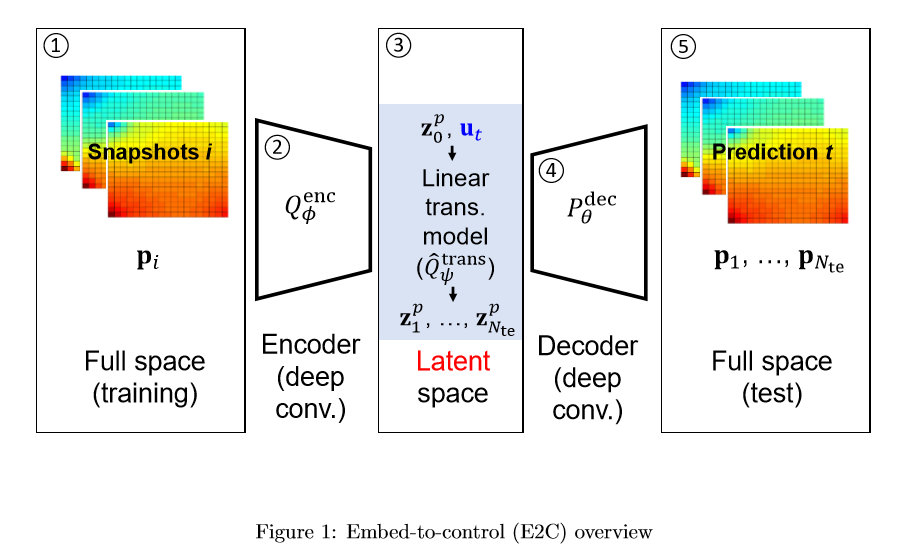
\includegraphics[width=8cm]{./cfig/one}\\
  \caption{Embed-to control(E2C) overview}\label{cfig:f1}
\end{figure}
\end{frame}

\begin{frame}[fragile]{3.1 Encoder component}
\indent During training, sequences of pressure and saturation snapshots are fed through the encoder network, and sequences of latent state variables $\mathbf{z}_{t}\in \mathbb{R}^{l_{z}}$ are generated.
\begin{figure}[H]
  \centering
  % Requires \usepackage{graphicx}
  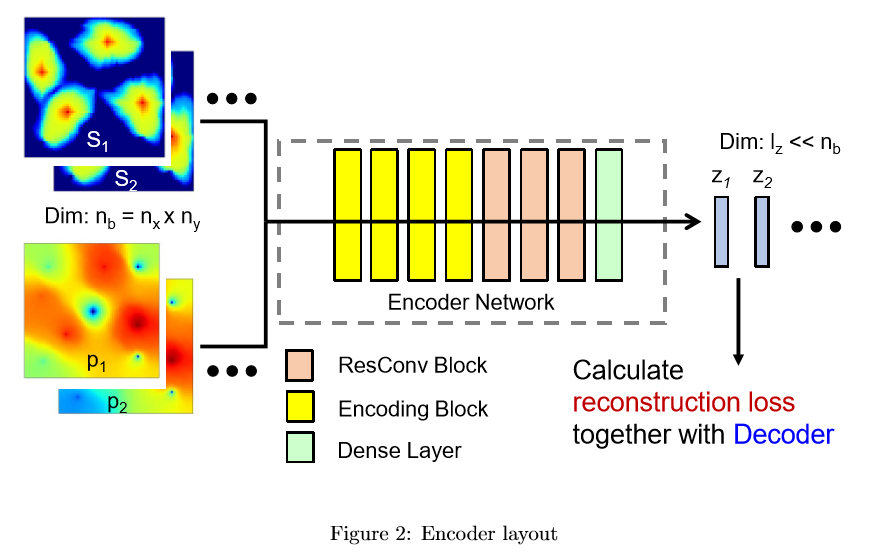
\includegraphics[width=8cm]{./cfig/two}\\
  \caption{Encoder layout}\label{cfig:f2}
\end{figure}
\end{frame}


\begin{frame}[fragile]{Appendix A}
\begin{figure}[H]
  \centering
  % Requires \usepackage{graphicx}
  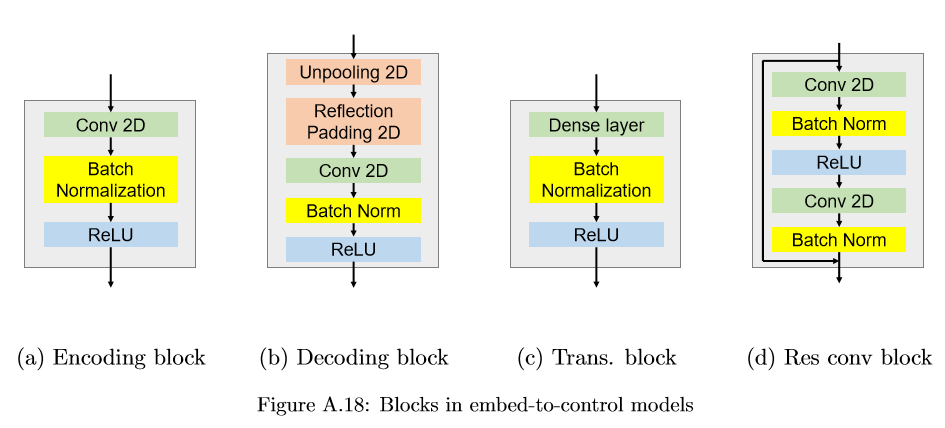
\includegraphics[width=12cm]{./cfig/three}\\
  \caption{Encoder layout}\label{cfig:fA.18}
\end{figure}
\end{frame}

\begin{frame}[fragile]{3.2 Encoder component}
The input to an encoding block is first fed through a convolution operation, which can also be viewed as a linear filter. The mathematical formulation of linear filtering is $F_{i, j}(\mathbf{x})=\sum_{p=-n}^{n} \sum_{q=-n}^{n} \mathbf{w}_{p, q} \mathbf{x}_{i+p, j+q}+b$ . A batchNorm operation is a crucial step in the efficient training of deep neural networks, since it renders the learning process less sensitive to parameter initialization, which means a larger initial learning rate can be used. ReLU is referred to as the 'activation' of the encoding block. The conv2D-batchNorm-ReLU architecture (with variation in ordering) is a standard processing step in CNNs.Following the idea of resNet, we add a stack of resConv blocks to the encoder network to deepen the network while mitigating the vanishing-gradient issue. A dense (fully-connected) layer is simply a linear projection that maps a high-dimensional vector to a low-dimensional vector.
\end{frame}

\begin{frame}[fragile]{3.3 Linear transition model}
\indent The inputs to the linear transition model include the latent variable for the current state $\mathbf{z}_{t}\in \mathbb{R}^{l_{z}}$  , the current step control $\mathbf{u}_{t+1}\in \mathbb{R}^{n_{w}}$  , and time step size $\Delta t$. The model outputs the predicted latent state for the next time step $\hat{\mathbf{Z}}_{t+1}$ .
\begin{figure}[H]
  \centering
  % Requires \usepackage{graphicx}
  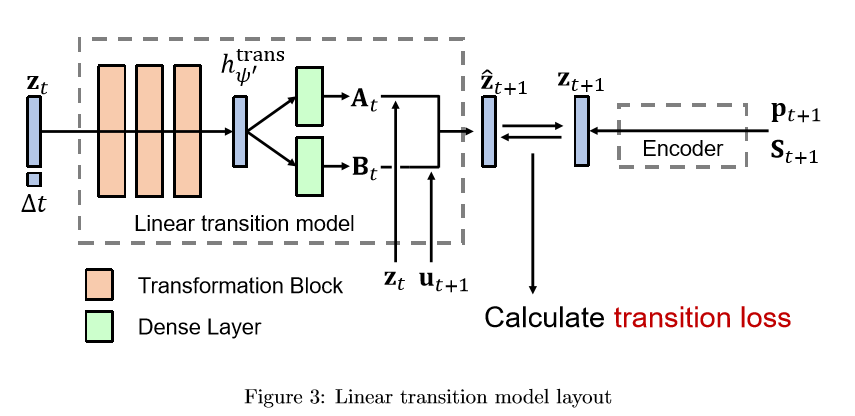
\includegraphics[width=8cm]{./cfig/four}\\
  \caption{Liner transition model layout}\label{cfig:f4}
\end{figure}
\end{frame}

\begin{frame}[fragile]{3.4 Decoder component}
\indent Latent variables predicted by the linear transition model (at time step t + 1) are fed to the decoder network as input, 15 and the predicted high-dimensional states are output. The architecture of the decoder is analogous to that of the encoder except it is in reversed order (which is not surprising since the decoder is conducting the inverse operation).
\begin{figure}[H]
  \centering
  % Requires \usepackage{graphicx}
  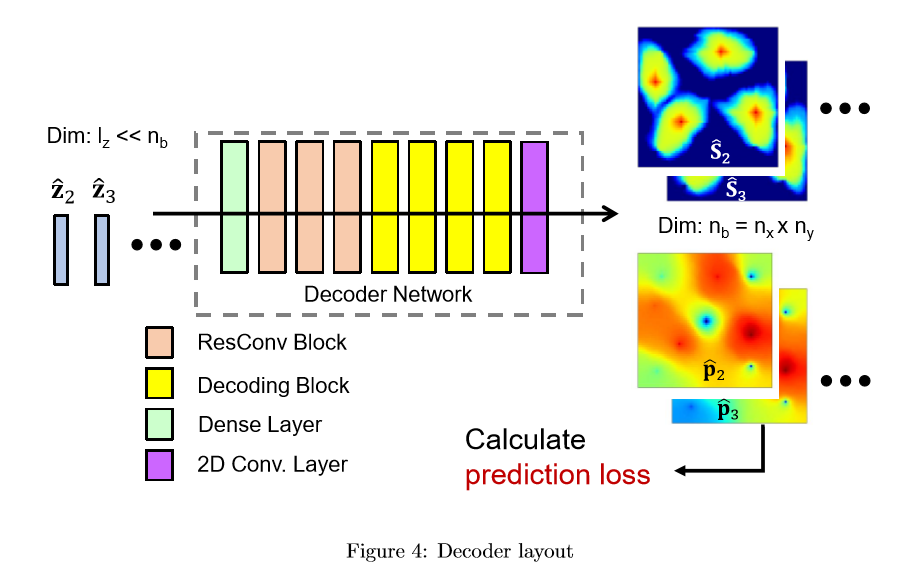
\includegraphics[width=6cm]{./cfig/five}\\
  \caption{Decoder layout}\label{cfig:f6}
\end{figure}
\end{frame}

\begin{frame}[fragile]{3.5 Loss function with physical constraints}

\indent We have briefly introduced the reconstruction loss $L_{R}$, the linear transition loss $L_{T}$, and the prediction loss $L_{PD}$, which comprise major components of the total loss function.\\
The reconstruction loss for a training data point $i$ can be expressed as :
\begin{equation}
\left(\mathcal{L}_{\mathrm{R}}\right)_{i}=\left\{\left\|\mathbf{x}_{t}-\hat{\mathbf{x}}_{t}\right\|_{2}^{2}\right\}_{i}
\end{equation}
The variable $x_{t}$ is the state variable at time step t from a training simulation, and$\hat{\mathbf{x}}_{t}=P_{\theta}^{\mathrm{dec}}\left(\mathbf{z}_{t}\right)=P_{\theta}^{\text {dec }}\left(Q_{\phi}^{\text {enc }}\left(\mathrm{x}_{t}\right)\right)$ denotes the states reconstructed by the encoder and decoder.\\
The linear transition loss for training point $i$ is similarly defined as
\begin{equation}
\left(\mathcal{L}_{\mathrm{T}}\right)_{i}=\left\{\left\|\mathbf{z}_{t+1}-\hat{\mathbf{z}}_{t+1}\right\|_{2}^{2}\right\}_{i}
\end{equation}
where $\mathbf{z}_{t+1}=Q_{\phi}^{\mathrm{enc}}\left(\mathbf{x}_{t+1}\right)$ is the latent variable encoded from the full-order state variable at $t+1$, and the variable $\hat{\mathbf{z}}_{t+1}=Q_{\psi}^{\text {trans }}\left(\mathbf{z}_{t}, \mathbf{u}_{t+1}, \Delta t\right)$ denotes the latent variable predicted by the linear transition model.

\end{frame}


\begin{frame}[fragile]{3.5 Loss function with physical constraints}
Finally, the prediction loss for training point $~i$ is defined as
\begin{equation}
\left(\mathcal{L}_{\mathrm{PD}}\right)_{i}=\left\{\left\|\mathbf{x}_{t+1}-\hat{\mathbf{x}}_{t+1}\right\|_{2}^{2}\right\}_{i}
\end{equation}
where $\mathbf{x}_{t+1}$ designates the state variable at time step t + 1 from the training simulations, and $\hat{\mathbf{x}}_{t+1}=P_{\theta}^{\mathrm{dec}}\left(\hat{\mathbf{z}}_{t+1}\right)$ represents the full-order state variable predicted by the ROM.\\
The data mismatch loss is the sum of these losses averaged over all training data points,
\begin{equation}
\mathcal{L}_{d}=\frac{1}{N_{t}} \sum_{i=1}^{N_{t}}\left(\mathcal{L}_{\mathrm{R}}\right)_{i}+\left(\mathcal{L}_{\mathrm{PD}}\right)_{i}+\lambda\left(\mathcal{L}_{\mathrm{T}}\right)_{i}
\end{equation}

We define the physics-based loss for each data point,as:
\begin{equation}
\begin{aligned}
\left(\mathcal{L}_{p}\right)_{i}=&\left\{\left\|\mathbf{k} \cdot\left[\left(\nabla \mathbf{p}_{t}-\nabla \hat{\mathbf{p}}_{t}\right)_{\text {recon }}+\left(\nabla \mathbf{p}_{t+1}-\nabla \hat{\mathbf{p}}_{t+1}\right)_{\text {pred }}\right]\right\|_{2}^{2}\right\}_{i} \\
&+\gamma\left\{\left\|\left(\mathbf{q}_{t}^{w}-\hat{\mathbf{q}}_{t}^{w}\right)_{\text {recon }}+\left(\mathbf{q}_{t+1}^{w}-\hat{\mathbf{q}}_{t+1}^{w}\right)_{\text {pred }}\right\|_{2}^{2}\right\}
\end{aligned}
\end{equation}
\end{frame}

\begin{frame}[fragile]{3.5 Loss function with physical constraints}
The physics-based loss function is computed by averaging $\left(\mathcal{L}_{p}\right)_{i}$ over all data points, i.e
\begin{equation}
\mathcal{L}_{p}=\frac{1}{N_{t}} \sum_{i=1}^{N_{t}}\left(\mathcal{L}_{p}\right)_{i}
\end{equation}
Combining the loss for data mismatch with this physics-based loss, the total loss function becomes
\begin{equation}
\mathcal{L}=\mathcal{L}_{d}+\alpha \mathcal{L}_{p}
\end{equation}
\end{frame}

\begin{frame}[fragile]{3.5 Loss function with physical constraints}
\begin{figure}[H]
  \centering
  % Requires \usepackage{graphicx}
  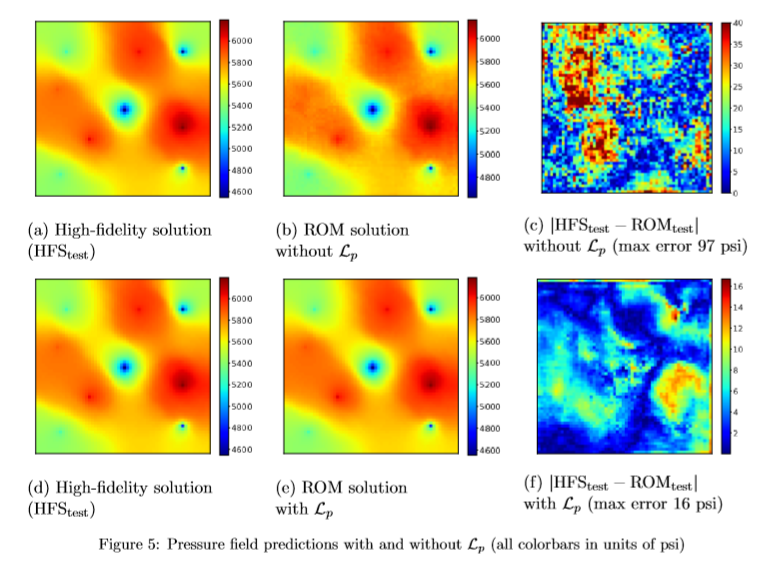
\includegraphics[width=8cm]{./cfig/six}\\
  \caption{Pressure field predictions with and without $\mathcal{L}_{p}$ }\label{cfig:f7}
\end{figure}
\end{frame}

%\begin{frame}[fragile]{3.6 E2C implementation and training details}

%\end{frame}
\section{Embed-to-control formulation}
\begin{frame}[fragile]{model setup}
\indent The geological model, in terms of the log-permeability field, is shown in Fig. 6. The locations of the four injection wells and five production wells are also displayed.
\begin{figure}[H]
  \centering
  % Requires \usepackage{graphicx}
  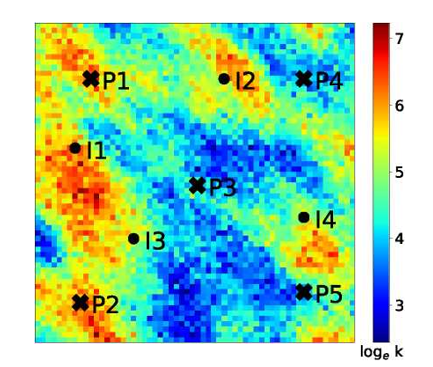
\includegraphics[width=8cm]{./cfig/seven}\\
  \caption{Log-permeability field and well locations}\label{cfig:f8}
\end{figure}
\end{frame}

\begin{frame}[fragile]{model setup}
\indent In the examples in this paper, we simulate a total of 300 training runs.Rather than train over all snapshots, here we set $N_{\mathrm{ctrl}}=N_{\mathrm{tr}}=N_{\mathrm{te}}=20$. This accelerates training and focuses ROM predictions on quantities of interest at time steps when the controls are changing. This results in a total number of data points of $N_{\mathrm{t}}=300\times20= 6000$.//
The gradient of the total loss function with respect to the model parameters $(\phi, \psi, \theta)$ is calculated via back-propagation through the embed-to-control framework. The adaptive moment estimation (ADAM) algorithm is used for this optimization, as it has been proven to be effective for optimizing deep neural networks.
\end{frame}


\end{CJK*}
\end{document}
